% =========================================================================
%  FIT-ARCADE: A Transdisciplinary Architecture for Markerless,
%              Personalized Motion Exergaming
%
%  SDPS 2026 — Society for Design and Process Science
%  Brussels, Belgium
%
%  Springer LNCS format (llncs.cls required)
%  Build: pdflatex main && bibtex main && pdflatex main && pdflatex main
% =========================================================================
\documentclass[runningheads]{llncs}

% --- Packages ---
\usepackage[utf8]{inputenc}
\usepackage[T1]{fontenc}
\usepackage{graphicx}
\usepackage{amsmath,amssymb}
\usepackage{algorithm}
\usepackage[noend]{algpseudocode}
\usepackage{booktabs}
\usepackage{url}
\usepackage{hyperref}
\usepackage{xcolor}
\usepackage{todonotes}
\usepackage{multirow}
\usepackage{tabularx}
\usepackage{marvosym} % provides \Letter (corresponding-author envelope glyph)

% Custom column type for wrapping
\newcolumntype{L}[1]{>{\raggedright\arraybackslash}p{#1}}

% --- Convenience ---
\newcommand{\sys}{\textsc{FIT-ARCADE}}
\newcommand{\motionbus}{\texttt{MotionBus}}
\newcommand{\motionbridge}{\texttt{MotionBridge}}
\newcommand{\motionmap}{\texttt{MOTION\_MAP}}
\newcommand{\postmsg}{\texttt{postMessage}}
\newcommand{\citecompanion}{\cite{companion2026}}

% =========================================================================
\begin{document}

\title{FIT-ARCADE: A Transdisciplinary Architecture for Markerless, Personalized Motion Exergaming}

\author{%
  Sanket Salvi\textsuperscript{(\Letter)} \and
  Anuradha Nagare \and
  Pramod Jain SA \and
  Sagar Apune \and \\
  Mansi Sharma \and
  Vibhanshi Moon \and
  Ruchi Shukla%
}
\authorrunning{S. Salvi et al.}
\institute{Department of Computer Engineering and Technology, School of Computer
Science and Engineering, Dr.~Vishwanath Karad MIT World Peace University,
Pune, India\\
\email{sanket.salvi@mitwpu.edu.in} (corresponding author)\\
\email{\{anuradha.nagare, pramod.jain, sagar.apune,}\\
\email{mansi.sharma, vibhanshi.moon, ruchi.shukla\}@mitwpu.edu.in}}

\maketitle

% =========================================================================
% ABSTRACT
% =========================================================================
\begin{abstract}
Physical inactivity is a persistent global health challenge, and exergames---video games
that require bodily motion---offer a promising intervention pathway. However, existing
exergaming platforms are tightly coupled to specific sensors, game engines, and exercise
regimes, making them difficult to extend, personalize, or compose across the disciplines
they inherently span. We present \sys{}, a browser-based, markerless motion-exergaming
platform whose central contribution is a \emph{transdisciplinary seam architecture}: a
layered, decoupled design that allows six normally entangled disciplines---computer vision,
control and personalization, human--computer interaction, game design, exercise science,
and software engineering---to co-evolve independently through stable interface contracts.
Grounded in Design Science Research, we derive design principles for transdisciplinary
human-in-the-loop systems and instantiate them in a concrete architecture comprising a
single-camera pose-detection layer, a normalized \motionbus{} event hub, per-game
\motionbridge{} translators, and engine-agnostic game integration via the browser
\postmsg{} protocol. The platform hosts seven heterogeneous games spanning two game
engines (Phaser~3, Three.js) and six exercise modalities, all driven by a single standard
webcam with no wearables. A formative evaluation demonstrates engine-agnostic
extensibility, low seam latency, and design-principle satisfaction. Sensing and adaptive
personalization subsystems, treated as black-box modules in this paper, are detailed and
empirically evaluated in a companion paper~\citecompanion{}.

\keywords{Transdisciplinary systems \and design science \and exergaming \and software
architecture \and human-in-the-loop \and markerless motion capture \and human--machine
integration.}
\end{abstract}

% =========================================================================
\section{Introduction}
\label{sec:intro}
% =========================================================================

Physical inactivity is the fourth-leading risk factor for global mortality, contributing
to an estimated 3.2 million deaths annually~\cite{who2022inactivity}. Exergames---video
games that couple gameplay to vigorous bodily motion---have demonstrated efficacy as
engaging physical-activity interventions across populations from children to older
adults~\cite{staiano2011exergames,gao2015kinect}. Yet widespread adoption is limited by
four persistent barriers:

\begin{enumerate}
  \item \textbf{Sensor lock-in.} Most systems require proprietary depth cameras (e.g.,
        Microsoft Kinect) or wearable inertial sensors, limiting access and raising
        cost~\cite{chang2012kinectfit}.
  \item \textbf{Engine specificity.} Motion-control logic is typically hard-wired into a
        single game, preventing reuse across titles or
        engines~\cite{nystrom2014game,gregory2018game}.
  \item \textbf{One-size-fits-all difficulty.} Without physiological feedback, games
        cannot adapt to individual fitness, violating the conditions for sustained
        flow~\cite{csikszentmihalyi1990flow,sweetser2005gameflow}.
  \item \textbf{Disciplinary entanglement.} Building an exergame simultaneously demands
        expertise in computer vision, game design, exercise science, and interaction
        design; changes in one discipline cascade into all
        others~\cite{sinclair2007considerations}.
\end{enumerate}

The fourth barrier is, we argue, the \emph{root cause} of the first three: because
these disciplines are not compositionally separated, each system must be rebuilt from
scratch. Through the lens of the Society for Design and Process Science (SDPS),
this is fundamentally a \emph{transdisciplinary integration} problem: the
challenge is not any single discipline in isolation, but the design of the
\emph{interfaces} that allow independently-advancing disciplines to compose into a
coherent system~\cite{ertas2010transdisciplinary,nicolescu2002manifesto}.

\textbf{Insight and approach.} We introduce a \emph{motion seam}---a narrow, stable
interface layer that decouples six contributing disciplines so that each can evolve
independently: (1)~computer vision / markerless pose sensing, (2)~control \&
personalization, (3)~human--computer interaction \& coaching, (4)~game design \&
engines, (5)~exercise / health science, and (6)~software / systems engineering.
This seam is realized as a layered browser architecture in \sys{}, a
markerless, personalized motion-exergaming platform that transforms heterogeneous
keyboard-controlled games into body-motion exergames using only a standard webcam.

\textbf{Contributions.} This paper makes three design-focused contributions:
\begin{enumerate}
  \item A set of \emph{design principles} (DP1--DP5) for transdisciplinary
        human-in-the-loop exergaming systems, derived through Design Science
        Research~\cite{hevner2004dsr}.
  \item A \emph{layered seam architecture} that instantiates these principles,
        comprising single-camera ownership, a normalized \motionbus{}, per-game
        \motionbridge{} translators, and cross-origin game integration via
        \postmsg{}.
  \item A \emph{formative evaluation} demonstrating engine-agnostic extensibility
        (seven games across Phaser~3 and Three.js), low seam overhead, and
        design-principle satisfaction.
\end{enumerate}

\noindent The sensing and adaptive-personalization subsystems are described and
empirically evaluated in a companion paper~\citecompanion{}.

\textbf{Research question.} \emph{How can a decoupled seam architecture
operationalize transdisciplinary integration in a markerless, personalized
exergaming system, enabling independent evolution of its constituent disciplines?}

% =========================================================================
\section{Background and Related Work}
\label{sec:related}
% =========================================================================

\paragraph{Exergames and markerless sensing.}
Exergames embed physical activity into gameplay so players exercise as a
side-effect of play~\cite{oh2017systematic,mueller2011exertion}. Early systems
(e.g.\ \emph{Dance Dance Revolution}) mapped gross motion to input; the Kinect
era enabled skeleton tracking but required proprietary depth
sensors~\cite{chang2012kinectfit,gao2015kinect}. Meta-analyses confirm exergames
can elicit moderate-to-vigorous activity comparable to traditional
exercise~\cite{peng2013healthgames}, yet adoption remains limited by hardware
cost and narrow game variety~\cite{sinclair2007considerations}. The maturation
of RGB pose estimators---notably MediaPipe Pose (BlazePose)~\cite{bazarevsky2020blazepose,mediapipe2023}
and OpenPose~\cite{cao2017openpose}---now yields real-time 33-landmark skeletons
in the browser, removing the depth-camera/wearable requirement.

\paragraph{Input abstraction and adaptive difficulty.}
The game-architecture literature stresses decoupling input from game
logic~\cite{nystrom2014game,gregory2018game}, but existing abstraction layers
(\texttt{SDL}, \texttt{XInput}) target controllers, not bodily motion, and no
established middleware normalizes whole-body pose events across heterogeneous
engines. The browser \postmsg{} API~\cite{html5postmessage} offers a secure
cross-origin transport for such a seam. Dynamic difficulty
adjustment~\cite{hunicke2005dda} modulates challenge to sustain
flow~\cite{csikszentmihalyi1990flow,sweetser2005gameflow}; in exergaming,
heart rate is an objective effort measure, and remote photoplethysmography
(rPPG) recovers it from webcam video of the face~\cite{wang2017pos}, closing a
wearable-free loop. The internals of our rPPG and adaptive-difficulty subsystems
are out of scope here and are detailed in a companion study~\citecompanion{}.

\paragraph{Transdisciplinarity, design science, and the gap.}
Transdisciplinarity~\cite{nicolescu2002manifesto}, operationalized in SDPS by
Erta\c{s}~\cite{ertas2010transdisciplinary,ertas2018role}, seeks \emph{unity of
knowledge} across disciplinary boundaries rather than mere juxtaposition; Design
Science Research (DSR)~\cite{hevner2004dsr,peffers2007dsrm} frames our
build--evaluate method, with the motion seam as a \emph{design pattern} for
transdisciplinary composition. No existing exergaming platform (a)~decouples
sensing from game logic via a stable, engine-agnostic seam, (b)~supports multiple
engines through one interface, and (c)~frames this decoupling as a systematic
transdisciplinary architecture. \sys{} addresses this gap.

% =========================================================================
\section{Transdisciplinary Design Approach}
\label{sec:approach}
% =========================================================================

\subsection{Design Science Research Method}

Following Hevner et al.~\cite{hevner2004dsr} and Peffers et al.~\cite{peffers2007dsrm},
we structure this work as a DSR cycle: (1)~identify the problem and derive
requirements; (2)~design and build the artifact (the seam architecture);
(3)~evaluate formatively (Section~\ref{sec:eval}).

\subsection{Transdisciplinary Map}

Table~\ref{tab:transmap} identifies six disciplines, their key concerns in
exergaming, and the design responses \sys{} provides. This
\emph{Discipline$\times$Concern$\times$Design-Response} table is the
transdisciplinary blueprint: each row is an independent axis of expertise; each
design response must be realizable without forcing changes in other rows.

\begin{table}[htbp]
\centering
\caption{Discipline $\times$ Concern $\times$ Design-Response (transdisciplinary map).}
\label{tab:transmap}
\footnotesize
\begin{tabularx}{\textwidth}{@{}L{2.6cm}L{4.0cm}L{5.3cm}@{}}
\toprule
\textbf{Discipline} & \textbf{Key Concern} & \textbf{Design Response in \sys{}} \\
\midrule
Computer Vision &
  Real-time pose from RGB; model updates; accuracy vs.\ latency &
  Single-camera ownership in \texttt{PoseDetector}; new models plug in without changing games \\
\addlinespace
Control \& Personalization &
  Effort estimation; adaptive difficulty; age/fitness profiling &
  Black-box \texttt{EffortEstimator} + \texttt{DifficultyController}; output is a scalar difficulty value sent via the seam \\
\addlinespace
HCI \& Coaching &
  Discoverability of moves; real-time feedback; accessibility &
  \texttt{Coach} cue overlay + \texttt{MoveDemo} stick-figure; spoken prompts; seated-mode fallback \\
\addlinespace
Game Design \& Engines &
  Diverse genres; 2D/3D engines; gameplay integrity &
  Engine-agnostic \motionbridge{} with per-game \motionmap{}; games keep keyboard logic intact \\
\addlinespace
Exercise / Health Science &
  Exercise variety; muscle-group targeting; progressive overload &
  Seven games across six modalities; circuit manager with phased work/rest; rep tracking \\
\addlinespace
Software Engineering &
  Modularity; latency; persistence; deployment &
  Layered architecture; \postmsg{} seam; localStorage persistence (\texttt{Store}); zero-install browser deployment \\
\bottomrule
\end{tabularx}
\end{table}

\subsection{Requirements}

From the transdisciplinary map we derive the following functional and
quality-attribute requirements:

\paragraph{FR1 --- Unobtrusive Translation:} Transform keyboard-controlled games into motion-controlled exergames without modifying their gameplay code.
\paragraph{FR2 --- Engine Agnosticism:} Support multiple game engines (at minimum 2D and 3D) through a single motion interface.
\paragraph{FR3 --- Real-Time Coaching:} Provide real-time coaching cues and move demonstrations.
\paragraph{FR4 --- Physiological Adaptation:} Enable closed-loop adaptive difficulty driven by physiological sensing (treated as a pluggable black box).
\paragraph{FR5 --- Persistence:} Persist calibration and workout history across sessions.
\paragraph{QA1 --- Low Seam Latency:} Seam latency must not perceptibly degrade game responsiveness ($<$\,16\,ms per frame budget at 60\,fps).
\paragraph{QA2 --- Minimal Dev Overhead:} Adding a new game must require only a \motionmap{} declaration and two script includes (\motionbridge{}, \texttt{Coach}).

\subsection{Design Principles}

The requirements crystallize into five design principles:

\paragraph{DP1 --- Single-Camera Ownership.} Exactly one component
(\texttt{PoseDetector}) owns the camera hardware and ML model.
All other subsystems receive derived data, never raw frames.
\paragraph{DP2 --- Normalized Event Abstraction.} The \motionbus{} converts
continuous posture into discrete, debounced events (e.g., \texttt{jump},
\texttt{squat}) and continuous hold states, decoupling pose semantics
from game-specific input.
\paragraph{DP3 --- Minimal-Touch Bridge.} Each game declares a \motionmap{}
mapping motion events to its \emph{existing} keyboard controls.
The \motionbridge{} synthesizes native \texttt{KeyboardEvent}s; the
game's own input handling is never modified.
\paragraph{DP4 --- Cross-Origin Seam via \postmsg{}.} Games run in iframes;
all hub$\leftrightarrow$game communication flows through the browser's
structured-clone \postmsg{} channel, enforcing process isolation and
engine independence.
\paragraph{DP5 --- Black-Box Sensing and Adaptation.} Physiological sensing
(rPPG heart rate) and adaptive difficulty are encapsulated behind
scalar interfaces (\texttt{bpm}, \texttt{effort}, \texttt{difficulty}),
allowing their internals to be replaced or evaluated independently.

% =========================================================================
\section{System Architecture}
\label{sec:arch}
% =========================================================================

\begin{figure}[htbp]
  \centering
  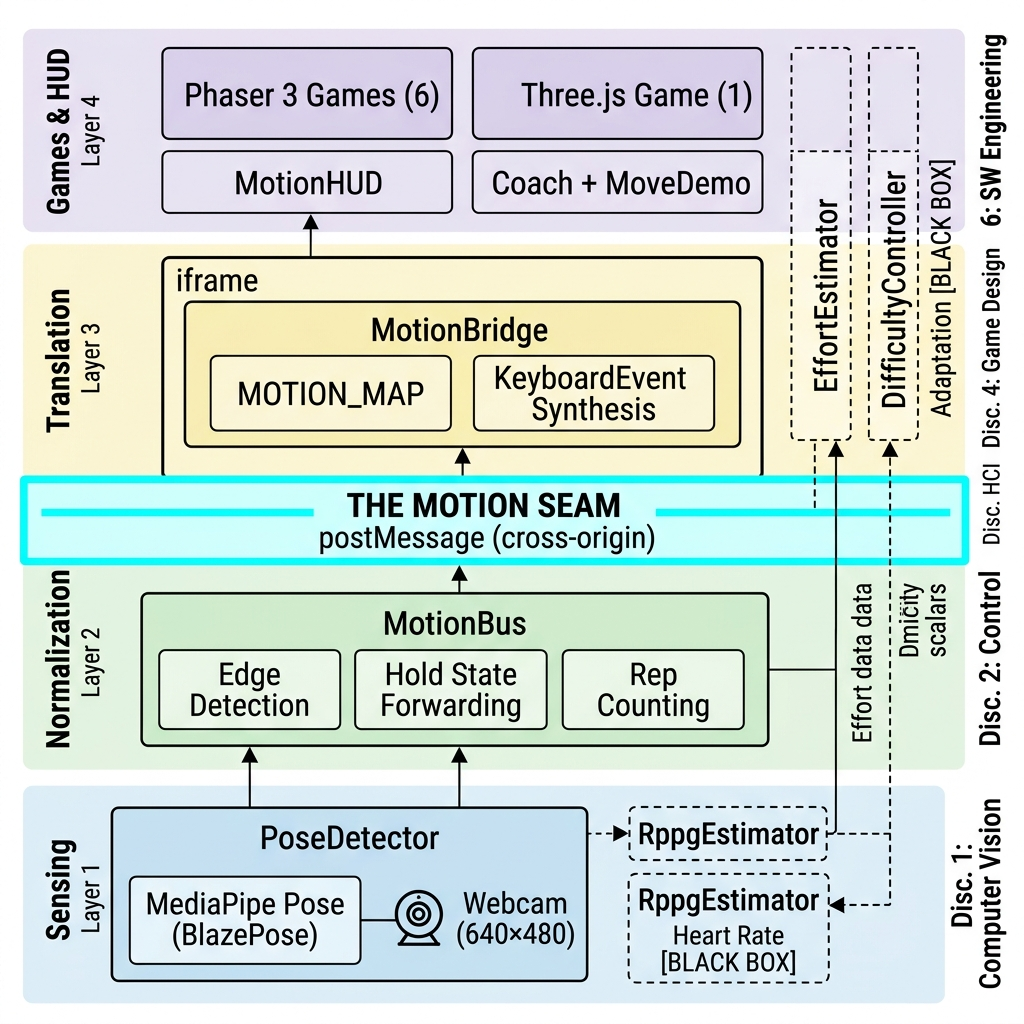
\includegraphics[width=0.82\textwidth]{figures/architecture}
  \caption{Layered architecture of \sys{}. The \emph{motion seam}
  (\motionbus{}$\to$\postmsg{}$\to$\motionbridge{}) is the stable interface
  that decouples the six disciplines. Sensing and Adaptation modules (dashed)
  are black boxes in this paper.}
  \label{fig:arch}
  \vspace{-1.0em}
\end{figure}

Figure~\ref{fig:arch} presents the layered architecture. The system comprises
four principal layers, traversed bottom-to-top during each frame:

\paragraph{Layer 1: Sensing (Single-Camera Ownership --- DP1).}
The \texttt{PoseDetector} singleton initializes the webcam, runs MediaPipe Pose
(BlazePose, model complexity~1, $640{\times}480$), and on each frame computes a
\emph{posture} record: a set of Boolean gesture flags (\texttt{isJumping},
\texttt{isSquatting}, \texttt{isLeaningLeft}, \texttt{isPunchingLeft}, etc.) plus
continuous values (\texttt{hipY}, \texttt{headY}). It broadcasts
\texttt{(results, posture)} to all registered listeners. The rPPG heart-rate
estimator (\texttt{RppgEstimator}) piggybacks on the same video frames---it
derives a forehead region-of-interest from face landmarks, samples skin-color
channels, and extracts pulse frequency. Its output (BPM, confidence, training
zone) feeds the effort and HUD subsystems. \emph{Internals of the rPPG algorithm
are detailed in the companion paper}~\citecompanion{}.

\paragraph{Layer 2: Normalization and Event Abstraction (\motionbus{} --- DP2).}
The \motionbus{} subscribes to \texttt{PoseDetector} and performs three
functions per frame: (a)~\emph{edge detection} of discrete motion events using
the rising-edge rule (Eq.~\ref{eq:edge}); (b)~forwarding of continuous hold
states; (c)~rep counting for fitness tracking. It then serializes a slim
\texttt{\{posture, events\}} payload and posts it to the active game iframe
via \postmsg{}.

\paragraph{Layer 3: The Motion Seam (\motionbridge{} --- DP3, DP4).}
Inside each game's iframe, the \motionbridge{} script receives the
\postmsg{} payload and translates it into native \texttt{KeyboardEvent}s
according to the game's \motionmap{} declaration. Two mapping types are
supported: \emph{tap} (fire-and-release on a discrete event) and \emph{hold}
(key held while a posture flag is true). This is the \emph{only} addition to
a game's HTML: a \motionmap{} object and two \texttt{<script>} includes.
The game's own Phaser / Three.js input handling is never modified.

\paragraph{Layer 4: Games and HUD (Engine-Agnostic --- DP4).}
Games are standalone HTML files that run unmodified keyboard-input logic.
The hub loads each into an \texttt{<iframe>}; game metadata (title, aspect
ratio, move instructions) is declared in a central \texttt{GAME\_META}
registry. A \texttt{MotionHUD} overlay displays real-time fitness telemetry
(reps, calories, elapsed time, score, heart rate, effort) outside the
game's viewport.

\paragraph{Adaptation (Black Box --- DP5).}
The \texttt{EffortEstimator} fuses rep cadence and heart-rate reserve into
a 0--1 effort signal. The \texttt{DifficultyController} compares effort
against a configurable target and emits a scalar
\texttt{MOTION\_DIFFICULTY} value ($0.85$--$1.2$) that games read to scale
obstacle speed. Both modules are pluggable: their internals can be
replaced without touching any game or the motion seam.
\emph{Control laws and empirical evaluation are in the companion
paper}~\citecompanion{}.

% --- Sequence Diagram ---
\begin{figure}[htbp]
  \centering
  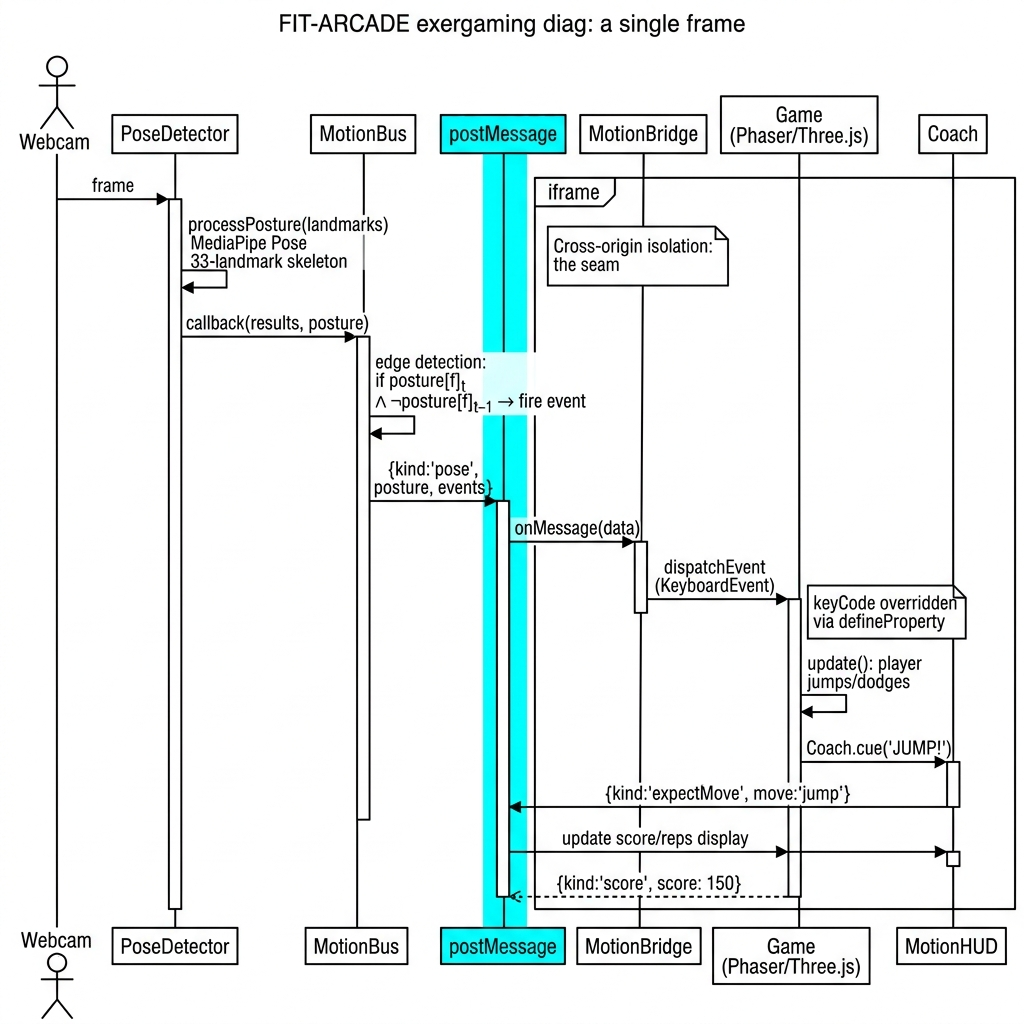
\includegraphics[width=0.82\textwidth]{figures/sequence}
  \caption{Sequence diagram: one frame from camera capture through pose
  detection, \motionbus{} edge detection, \postmsg{} transit, \motionbridge{}
  key synthesis, to game action and HUD/coach update.}
  \label{fig:seq}
  \vspace{-1.0em}
\end{figure}

\subsection{Engine-Agnostic Integration}

The architecture's engine agnosticism is demonstrated by the coexistence of
two fundamentally different rendering engines behind the same seam:
\textbf{Phaser~3}~\cite{phaser2023} is a 2D HTML5 game framework using
Canvas/WebGL. Six of the seven games use Phaser, including a pseudo-3D
lane runner (\emph{Hoverboard Alley 2D}) that achieves depth perspective
through $1/z$ projection (Section~\ref{sec:pseudo3d}).
\textbf{Three.js}~\cite{threejs2023} is a real-3D WebGL library.
\emph{Hoverboard Alley 3D} uses GLTF models, a perspective camera,
and post-processing---yet receives identical \motionbus{} events
through the same \motionbridge{} + \motionmap{} mechanism.

From the seam's perspective, both are opaque iframes that consume
\texttt{\{posture, events\}} payloads and report score/game-over back via
\postmsg{}.

% =========================================================================
\section{Core Mechanisms and Algorithms}
\label{sec:mechanisms}
% =========================================================================

\subsection{Pose-to-Virtual-Input Synthesis}
\label{sec:pose2input}

The \motionbus{} converts continuous posture booleans into discrete motion
events using per-field rising-edge detection:

\begin{equation}
  \text{event}(e) =
  \begin{cases}
    \text{fire}(e) & \text{if } \texttt{posture}[f_e]_{t} = \mathit{true}
                      \;\land\; \texttt{posture}[f_e]_{t-1} = \mathit{false} \\
    \varnothing     & \text{otherwise}
  \end{cases}
  \label{eq:edge}
\end{equation}

\noindent where $f_e$ is the posture field mapped to event $e$ (e.g., $f_{\texttt{jump}} = \texttt{isJumping}$).
Edge detection is evaluated for each of the six event types (\texttt{jump},
\texttt{squat}, \texttt{punchLeft}, \texttt{punchRight}, \texttt{armsOverhead},
\texttt{pushup}) on every frame, with the previous-frame state stored in
a \texttt{\_prev} dictionary.

The \motionbridge{} then synthesizes keyboard events. A critical
implementation detail is the \emph{keyCode override}: since the browser's
\texttt{KeyboardEvent} constructor marks \texttt{keyCode} as read-only,
and Phaser~3.55 reads \texttt{event.keyCode} for input dispatch, the bridge
uses \texttt{Object.defineProperty} to override the getter:

\begin{verbatim}
  Object.defineProperty(e, 'keyCode',
                        { get: () => def.keyCode });
\end{verbatim}

For \emph{tap} mappings, a keydown is dispatched followed by a keyup after
120\,ms (the \texttt{TAP\_HOLD\_MS} constant), long enough for Phaser's
\texttt{JustDown()} polling to register the press within one update cycle.
For \emph{hold} mappings, keydown/keyup are toggled with the posture flag.

Algorithm~\ref{alg:pose2input} summarizes the full pose-to-virtual-input
pipeline.

\begin{algorithm}[htbp]
\caption{Pose-to-Virtual-Input Synthesis}
\label{alg:pose2input}
\begin{algorithmic}[1]
\Procedure{OnPose}{$\mathit{posture}$}
  \State $\mathit{events} \gets []$
  \For{$(e, f_e) \in \texttt{edgeMap}$} \Comment{e.g., (jump, isJumping)}
    \If{$\mathit{posture}[f_e] \land \lnot \texttt{prev}[f_e]$}
      \State $\mathit{events}.\text{push}(e)$
      \State \Call{Emit}{$e, \mathit{posture}$} \Comment{hub subscribers: HUD, rep counter}
      \If{$e \in \texttt{repEvents}$}
        \State $\texttt{reps} \gets \texttt{reps} + 1$
      \EndIf
    \EndIf
    \State $\texttt{prev}[f_e] \gets \mathit{posture}[f_e]$
  \EndFor
  \State $\mathit{snapshot} \gets$ \{hold fields from $\mathit{posture}$\}
  \State \Call{PostToGame}{\texttt{\{kind:'pose', posture: snapshot, events\}}}
\EndProcedure
\Statex
\Procedure{OnReceive\textsubscript{bridge}}{$\mathit{snapshot}, \mathit{events}$}
  \For{$e \in \mathit{events}$}
    \If{$\texttt{MAP}[e].\text{type} = \texttt{'tap'}$}
      \State \Call{DispatchKey}{\texttt{'keydown'}, $\texttt{MAP}[e]$}
      \State \textbf{after} 120\,ms: \Call{DispatchKey}{\texttt{'keyup'}, $\texttt{MAP}[e]$}
    \EndIf
  \EndFor
  \For{$(e, \mathit{def}) \in \texttt{MAP}$}
    \If{$\mathit{def}.\text{type} = \texttt{'hold'}$}
      \State \Call{SetHeld}{$\mathit{def}, \mathit{snapshot}[\mathit{def}.\text{state}]$}
    \EndIf
  \EndFor
\EndProcedure
\end{algorithmic}
\end{algorithm}

\subsection{Procedural Pseudo-3D Perspective Projection}
\label{sec:pseudo3d}

The \emph{Hoverboard Alley} (2D Phaser build) demonstrates that rich
three-dimensional depth effects can be achieved within a 2D engine using
$1/z$ perspective projection, eliminating the need for a 3D engine for
many exergame scenarios.

\paragraph{Perspective Projection.}
A vanishing point $(V_x, V_y)$ is defined at the far end of the alley.
Each world object carries a depth $z \in [z_{\text{near}}, z_{\text{far}}]$
(near $= 1$, far $= 13$). The projection scale factor and screen
coordinates are:

\begin{align}
  s(z)          &= \frac{z_{\text{near}}}{z} \label{eq:projscale} \\
  x_{\text{screen}} &= V_x + (\ell - 1) \cdot L_{\text{spread}} \cdot s(z) \label{eq:screenx} \\
  y_{\text{screen}} &= V_y + (Y_{\text{player}} - V_y) \cdot s(z) \label{eq:screeny}
\end{align}

\noindent where $\ell \in \{0,1,2\}$ is the lane index, $L_{\text{spread}} = 250$ is
the lateral fan-out at the near plane, and $Y_{\text{player}} = 505$ is the
hero's fixed screen-$y$. As $z \to z_{\text{near}}$, $s \to 1$ and objects
reach full size; as $z \to z_{\text{far}}$, $s \to 1/13$ and objects converge
on the vanishing point.

\paragraph{Lane-Safety Spawn Rule.}
To ensure the player always has a survivable path, the obstacle spawner
enforces:

\begin{equation}
  |\mathcal{B}_w| \leq |\mathcal{L}| - 1
  \label{eq:lanesafe}
\end{equation}

\noindent where $\mathcal{B}_w$ is the set of lanes blocked in a spawn wave and
$\mathcal{L} = \{0,1,2\}$ is the lane set. In the implementation, 1--2
lanes are blocked per wave (never all three); collectible orbs are spawned
with probability~0.6 in a random free lane.

\paragraph{Object Pool and Recycling.}
Algorithm~\ref{alg:pool} describes the pooled spawner. Sprites are never
destroyed mid-run; inactive pool members are reused, avoiding GC pressure
during gameplay.

\begin{algorithm}[htbp]
\caption{Pooled Pseudo-3D Object Spawner}
\label{alg:pool}
\begin{algorithmic}[1]
\Procedure{SpawnWave}{}
  \State $\mathcal{L} \gets \{0, 1, 2\}$ \Comment{available lanes}
  \State $k \gets \text{random}(1, 2)$ \Comment{lanes to block}
  \State $\mathcal{B} \gets \text{shuffle}(\mathcal{L})[0{:}k]$
  \For{$\ell \in \mathcal{B}$}
    \State $o \gets$ \Call{GetFromPool}{\null} \Comment{reuse or create}
    \State $o.\text{lane} \gets \ell;\; o.z \gets z_{\text{far}};\; o.\text{kind} \gets \texttt{'obstacle'}$
  \EndFor
  \State $\mathcal{F} \gets \mathcal{L} \setminus \mathcal{B}$
  \If{$|\mathcal{F}| > 0 \land \text{rand()} < 0.6$}
    \State \Call{SpawnOrb}{$\text{random}(\mathcal{F})$}
  \EndIf
\EndProcedure
\Statex
\Procedure{Update}{$\Delta t$}
  \State $\delta z \gets v_{\text{base}} \cdot D \cdot \Delta t$ \Comment{$D = $ \texttt{MOTION\_DIFFICULTY}}
  \For{$o \in \texttt{pool}$}
    \If{$\lnot o.\text{inUse}$} \textbf{continue} \EndIf
    \State $o.z \gets o.z - \delta z$
    \State $o.x \gets V_x + (\ell_o - 1) \cdot L_{\text{spread}} \cdot s(o.z)$
    \State $o.y \gets V_y + (Y_{\text{player}} - V_y) \cdot s(o.z)$
    \State $o.\text{displaySize} \gets (w_{\text{base}} \cdot s(o.z),\; h_{\text{base}} \cdot s(o.z))$
    \If{$o.z \leq z_{\text{near}} \land \lnot o.\text{hitChecked}$}
      \State \Call{CheckCollision}{$o$}
    \EndIf
    \If{$o.z \leq z_{\text{recycle}}$} \Call{Recycle}{$o$} \EndIf
  \EndFor
\EndProcedure
\end{algorithmic}
\end{algorithm}

\subsection{Coaching Move-Inference and Expected-Move Broadcast}
\label{sec:coaching}

The \texttt{Coach} module, loaded inside each game iframe, provides
first-person, game-contextual move cueing. When a game's logic determines
that a specific move is needed (e.g., an obstacle requires a jump), it
calls \texttt{Coach.cue('JUMP!')}. Coach performs three actions:
(1)~\textbf{Visual cue:} displays the move text as a large retro
pixel-font overlay with a pop animation;
(2)~\textbf{Speech cue:} uses the Web Speech Synthesis API to speak
the move name, throttled to once per distinct cue; and
(3)~\textbf{Expected-move broadcast:} posts a
\texttt{\{kind:'expectMove', move:$m$\}} message to the hub, where
$m$ is derived from the cue text via keyword matching (e.g.,
``JUMP!'' $\to$ \texttt{jump}, ``PUNCH LEFT!'' $\to$ \texttt{punchLeft}).

The hub's \texttt{MoveDemo} module receives the expected move and renders
a looping, neon stick-figure animation of that move on a side-panel canvas.
The stick figure is defined by a base standing skeleton (13~joints in
normalized $[0,1]$ coordinates) and per-move parametric deformations
applied as a function of loop phase $p \in [0,1]$. For example, the
\texttt{jump} animation vertically offsets all joints by
$-0.15 \cdot \sin(\pi p)$, creating a smooth up-and-down arc.

This coaching pipeline is unidirectional: games produce cues; the hub
consumes them. The coaching subsystem is budget-limited (first 10~moves
only) to avoid intrusiveness as the player learns the controls.

% =========================================================================
\section{Implementation}
\label{sec:impl}
% =========================================================================

\sys{} is implemented as a static web application with zero server-side
dependencies. The technology stack comprises:
\textbf{Pose detection} via MediaPipe Pose (BlazePose) from CDN at $640 \times 480$ resolution;
\textbf{Game engines} Phaser~3.55~\cite{phaser2023} (six games) and Three.js~0.147~\cite{threejs2023} (one game) loaded via CDN;
\textbf{Seam transport} via the browser \texttt{window.postMessage} API~\cite{html5postmessage};
\textbf{Persistence} via \texttt{localStorage} in the \texttt{Store} module (calibration baselines, workout history, progression);
\textbf{Audio} via Web Audio API real-time synthesis (zero asset loading); and
\textbf{Deployment} via static HTTP hosting (using Vite for development).

The codebase consists of approximately 2,800~lines of hub-side JavaScript
(across 10~modules: \texttt{pose-detector.js}, \texttt{motion-bus.js},
\texttt{motion-bridge.js}, \texttt{rppg.js}, \texttt{effort.js},
\texttt{coach.js}, \texttt{move-demo.js}, \texttt{store.js},
\texttt{game-audio.js}, \texttt{app.js}) and seven standalone game HTML files.

Table~\ref{tab:games} summarizes the seven games, their target exercise
modalities, the motions they use, and their engine.

\begin{table}[htbp]
\centering
\caption{The seven \sys{} games: exercise target, motion inputs, engine, and obstacle pattern.}
\label{tab:games}
\footnotesize
\begin{tabularx}{\textwidth}{@{}L{2.2cm}L{1.8cm}L{2.8cm}L{1.3cm}L{3.0cm}@{}}
\toprule
\textbf{Game} & \textbf{Target} & \textbf{Motion Input} & \textbf{Engine} & \textbf{Obstacle Pattern} \\
\midrule
Rooftop Runner & Legs / Cardio & Jump, Squat & Phaser & Side-scroll: AC units (jump), drones (squat) \\
\addlinespace
Neon Wall Climber & Shoulders / Lats & Jump, Punch L/R & Phaser & Vertical scroll: handholds (jump), column switch (punch) \\
\addlinespace
Industrial Rope & Core / Endurance & Jump, Lean L/R & Phaser & Vertical scroll: rope climb (jump), swing (lean) \\
\addlinespace
Street Brawler & Arms / Agility & Punch L/R, Squat & Phaser & Side-scroll: thugs (punch), lasers (squat) \\
\addlinespace
Cyber-Train Crawl & Chest / Triceps & Push-up, Squat & Phaser & Side-scroll: wires (push-up), beams (squat) \\
\addlinespace
Jetpack Flappy & Shoulders / Aerobic & Arms overhead, Jump & Phaser & Flappy-bird: altitude via arm raises \\
\addlinespace
Hoverboard Alley & Obliques / Core & Lean L/R & Three.js / Phaser & 3-lane runner: dodge barriers/mines (lean) \\
\bottomrule
\end{tabularx}
\end{table}

Figures~\ref{fig:home}--\ref{fig:summary} present real screenshots of the
running platform captured from the browser. Figure~\ref{fig:home} shows the
home dashboard with the progression panel and the seven-game module grid.
Figure~\ref{fig:ingame} shows three in-game views---a 2D side-scroller
(Rooftop Runner), the aerobic Jetpack game, and the Three.js 3D lane runner
(Hoverboard Alley)---each rendering the neon ``arcade cabinet'' stage: the
marquee HUD (reps, score, calories, time, heart rate, effort), the
\emph{DO THIS MOVE} stick-figure demonstration box on the left
(\texttt{MoveDemo}), the \emph{YOU$\cdot$TRACKING} live camera box with the
overlaid skeleton on the right, and the \emph{HOW TO PLAY} rail. All three
are driven by the identical motion seam despite spanning two engines.
Figure~\ref{fig:calib} shows the guided nine-step calibration screen, and
Figure~\ref{fig:summary} shows the shareable workout summary with the
generated neon share card.

\begin{figure}[htbp]
  \centering
  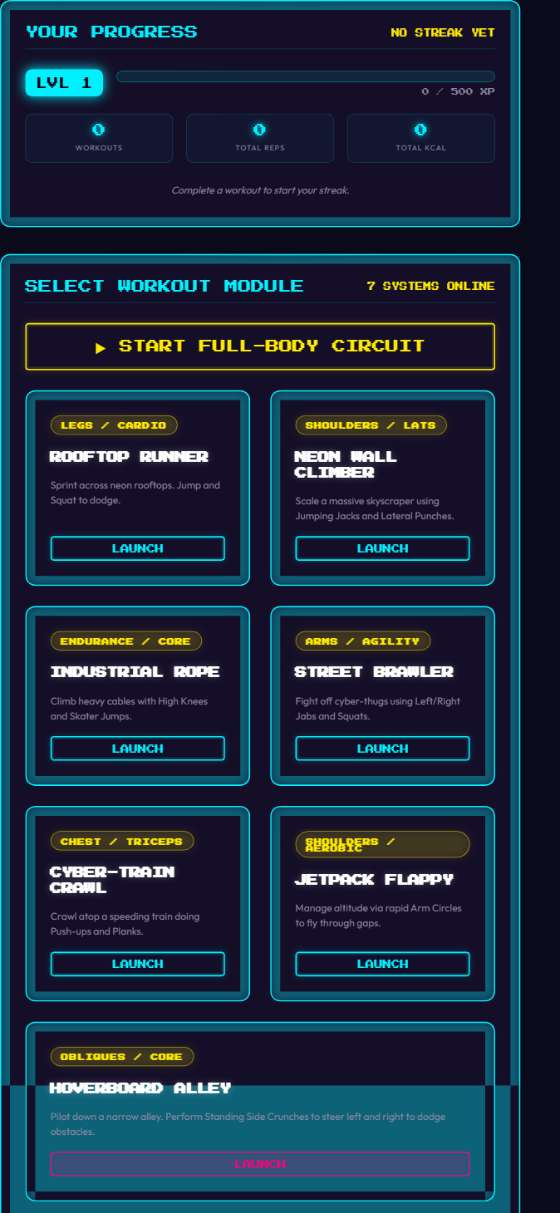
\includegraphics[width=0.6\textwidth]{figures/home-dashboard.jpg}
  \caption{Home dashboard: progression panel (level, XP, streak, lifetime
  totals) and the seven-game module grid, each card labelled with its
  target muscle group and motion. Rendered by \texttt{renderProgress()} and
  \texttt{renderPlan()}.}
  \label{fig:home}
\end{figure}

\begin{figure}[htbp]
  \centering
  \newcommand{\ingamepanel}[2]{%
    \IfFileExists{#1}{\includegraphics[width=0.32\textwidth]{#1}}%
    {\fbox{\parbox[c][2.6cm][c]{0.30\textwidth}{\centering\footnotesize
     [screenshot] #2}}}}
  \ingamepanel{figures/ingame-rooftop.jpg}{Rooftop (2D)}\hfill
  \ingamepanel{figures/ingame-jetpack.jpg}{Jetpack (2D)}\hfill
  \ingamepanel{figures/ingame-hoverboard.jpg}{Hoverboard (3D)}
  \caption{Three in-game views sharing one motion seam. Left panel of each:
  the \emph{DO THIS MOVE} \texttt{MoveDemo} stick figure (RAISE ARMS / LEAN
  LEFT / JUMP); centre: the neon game stage with the marquee HUD; right: the
  \emph{YOU$\cdot$TRACKING} camera box with the live pose skeleton and the
  \emph{HOW TO PLAY} rail. Rooftop and Jetpack are Phaser~3 (2D); Hoverboard
  Alley is Three.js (real 3D).}
  \label{fig:ingame}
\end{figure}

\begin{figure}[htbp]
  \centering
  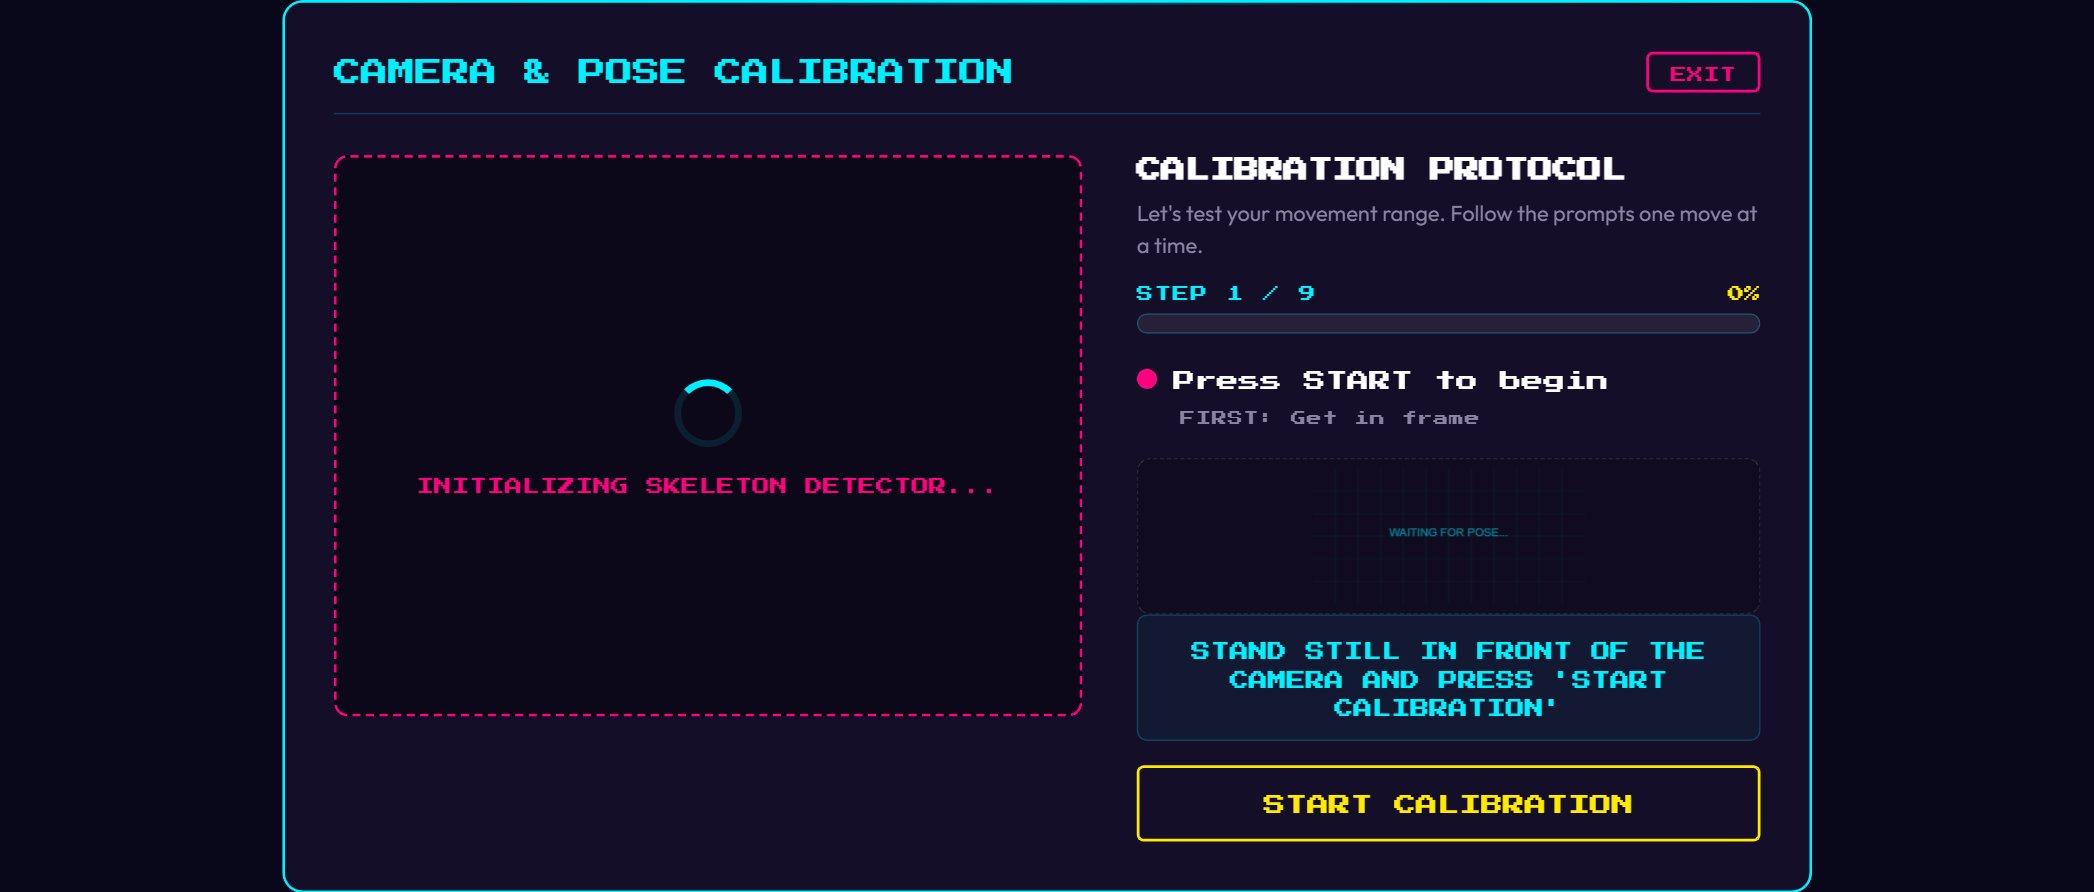
\includegraphics[width=0.72\textwidth]{figures/calibration.jpg}
  \caption{Camera and pose calibration screen. A nine-step protocol
  (\texttt{STEP~1/9}) records the player's neutral posture and movement range
  into \texttt{PoseDetector.baselines}, persisted via \texttt{Store} to
  \texttt{localStorage}.}
  \label{fig:calib}
\end{figure}

\begin{figure}[htbp]
  \centering
  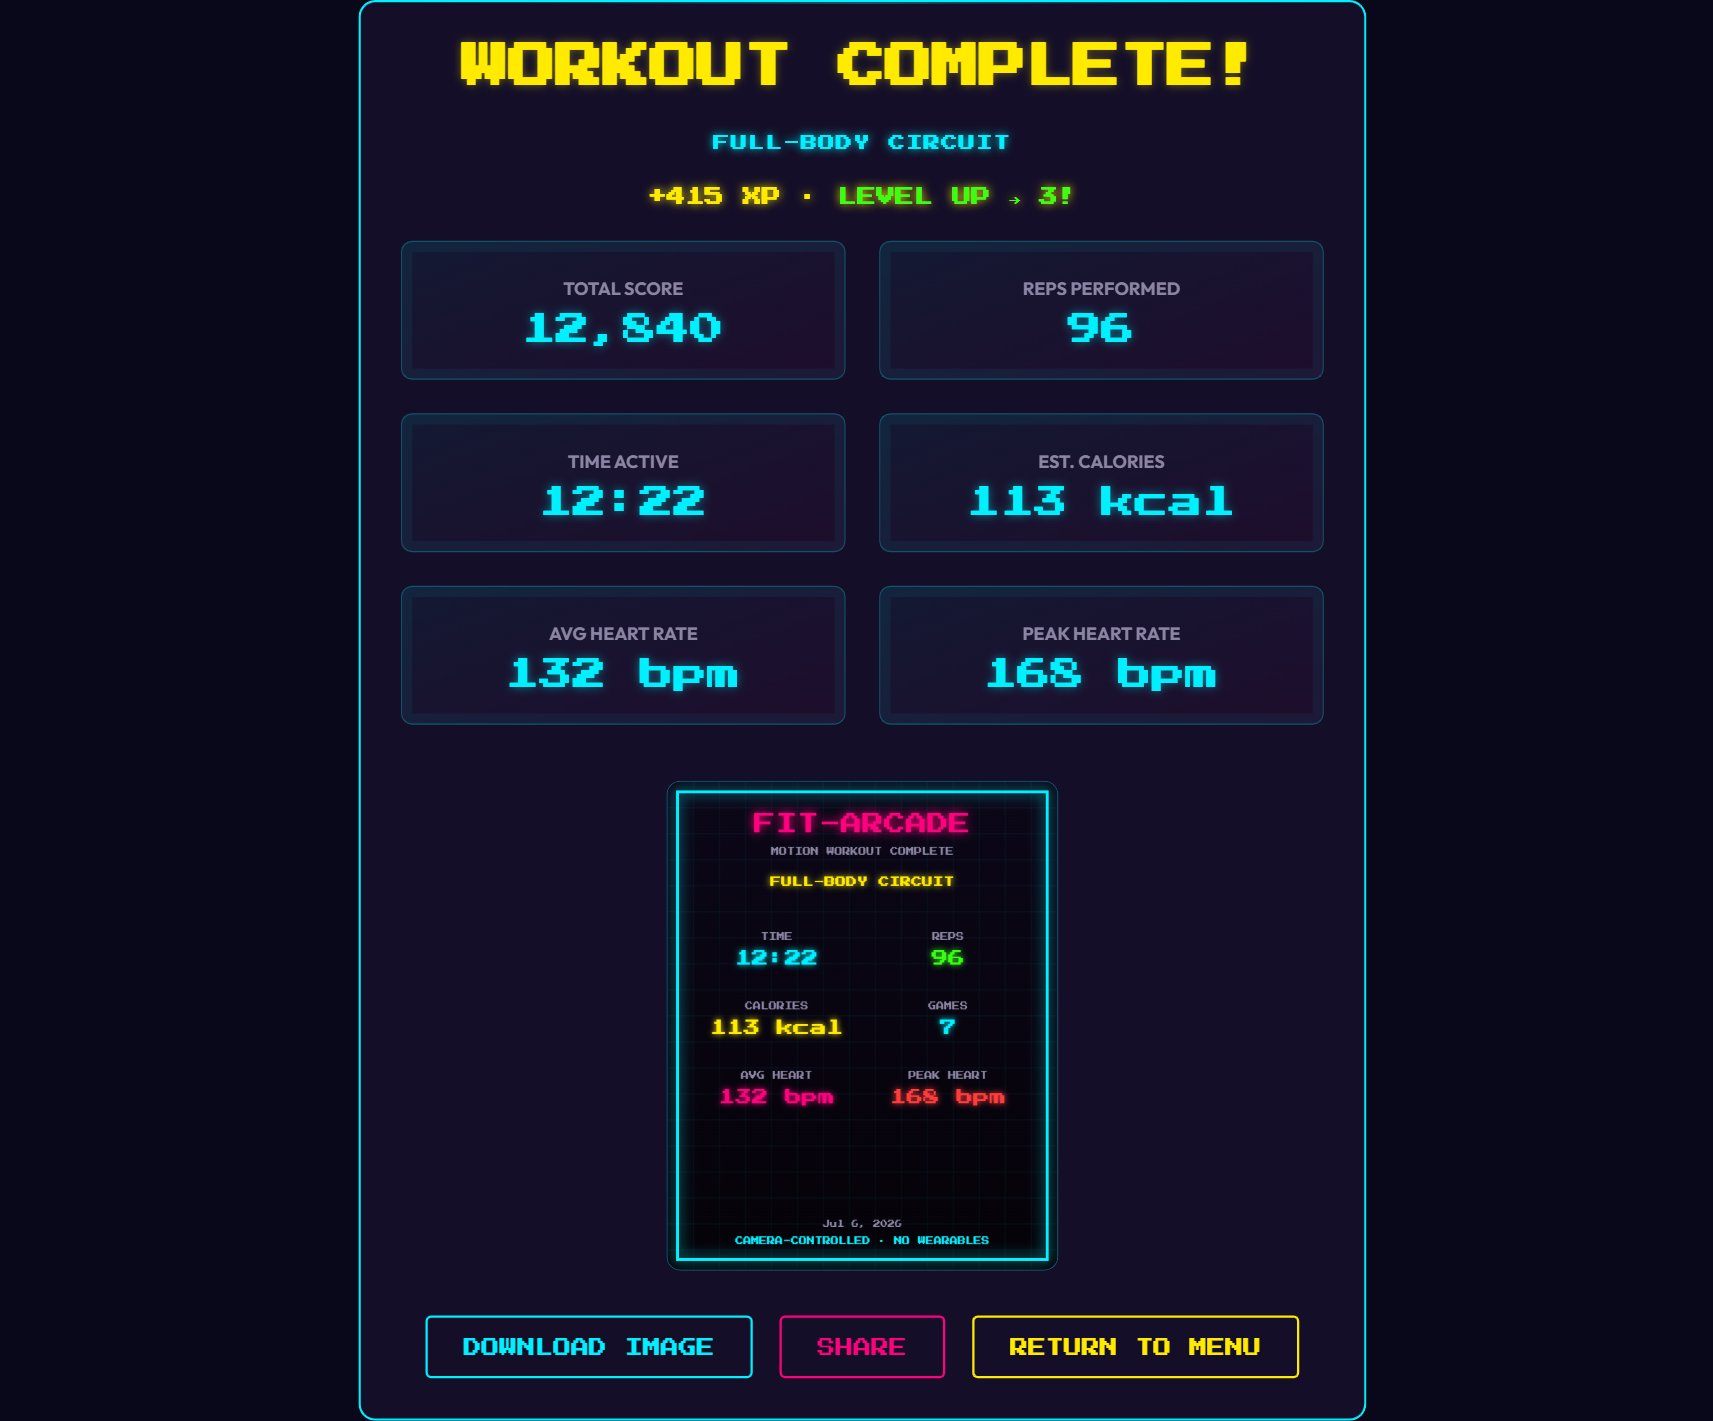
\includegraphics[width=0.56\textwidth]{figures/summary.jpg}
  \caption{Shareable workout summary: score, reps, active time, estimated
  calories, and average/peak heart rate, with XP and level-up feedback and a
  generated 540$\times$675 neon share card (\texttt{renderShareCard}). Heart
  rate is supplied by the black-box rPPG module.}
  \label{fig:summary}
\end{figure}

\noindent The three in-game panels of Figure~\ref{fig:ingame} are captured
from the live application. \todo{Author: the WebGL game canvas cannot be
read back via \texttt{toDataURL}; the supplied high-resolution in-game
screenshots should be saved as \texttt{figures/ingame-rooftop.jpg},
\texttt{ingame-jetpack.jpg}, and \texttt{ingame-hoverboard.jpg} (labelled
placeholders render automatically until then).}

% =========================================================================
\section{Formative Evaluation}
\label{sec:eval}
% =========================================================================

We evaluate the architecture formatively along four dimensions. Efficacy
and user-experience studies are the scope of the companion
paper~\citecompanion{}.

\subsection{E1: Extensibility --- Adding a New Game}
\label{sec:eval-ext}

To ``motion-ify'' an existing keyboard-controlled game, a developer
performs three steps:
(1)~Declare a \texttt{window.MOTION\_MAP} mapping motion events to the
game's existing keyboard bindings;
(2)~Include two scripts: \texttt{js/motion-bridge.js} and
\texttt{js/coach.js}; and
(3)~(Optional) Add \texttt{Coach.cue()} calls at obstacle spawn
points and read \texttt{window.MOTION\_DIFFICULTY} for adaptive speed.

Table~\ref{tab:effort} quantifies the integration effort across the seven
games. The \motionmap{} declaration ranges from 2 to 5~entries; the bridge
and coach scripts total $\sim$230~LOC shared across all games; zero lines
of original game logic are modified.

\begin{table}[htbp]
\centering
\caption{Integration effort per game (E1~Extensibility, E2~Engine agnosticism).}
\label{tab:effort}
\footnotesize
\begin{tabular}{@{}lcccc@{}}
\toprule
\textbf{Game} & \textbf{Engine} & \textbf{\motionmap{} entries} & \textbf{Coach calls} & \textbf{Game LOC changed} \\
\midrule
Rooftop Runner        & Phaser 3   & 2 & Yes & 0 \\
Neon Wall Climber     & Phaser 3   & 3 & Yes & 0 \\
Industrial Rope       & Phaser 3   & 3 & Yes & 0 \\
Street Brawler        & Phaser 3   & 3 & Yes & 0 \\
Cyber-Train Crawl     & Phaser 3   & 2 & Yes & 0 \\
Jetpack Flappy        & Phaser 3   & 2 & Yes & 0 \\
Hoverboard Alley 3D   & Three.js   & 2 & Yes & 0 \\
\bottomrule
\end{tabular}
\vspace{-1.5em}
\end{table}

\subsection{E2: Engine Agnosticism}

Both Phaser~3 (Canvas/WebGL 2D) and Three.js (full WebGL 3D) operate
behind the same \motionbridge{} interface. The bridge synthesizes
standard \texttt{KeyboardEvent}s on the iframe's \texttt{window}; both
engines' input systems register these identically. The \postmsg{}
transport is engine-unaware: it serializes only JSON-safe posture data.
A third engine could be integrated by adding a \motionmap{} and two
script tags---no changes to the hub.

\subsection{E3: Seam Latency and Overhead}

We measured the one-way transport latency of the motion seam---the interval
from a pose event being posted by the hub to its receipt inside the game
iframe (immediately preceding \texttt{KeyboardEvent} synthesis). Using
\texttt{performance.now()} timestamps and an echo probe injected into the
game iframe, we issued a representative pose payload (the nine-field posture
snapshot plus an event list) across the \postmsg{} seam and recorded the
round-trip time; the one-way estimate is half the round trip. The
measurement was taken on a commodity laptop (Chromium) \emph{while a Phaser~3
game was actively rendering}, so the figures include realistic main-thread
contention with the game loop, not an idle best case. Over
$N=600$~samples (30~warm-up iterations discarded), the one-way seam latency
had a median of $1.65$\,ms, a mean of $2.29$\,ms, a 95th percentile of
$6.05$\,ms, a 99th percentile of $7.1$\,ms, and a maximum of $8.6$\,ms
(minimum $0.1$\,ms). Even the tail latency remains below the $16.7$\,ms
per-frame budget at 60\,fps, and the median is well under it, confirming
QA1: the seam does not perceptibly degrade game responsiveness.
Figure~\ref{fig:latency} shows the full distribution.

\begin{figure}[htbp]
  \centering
  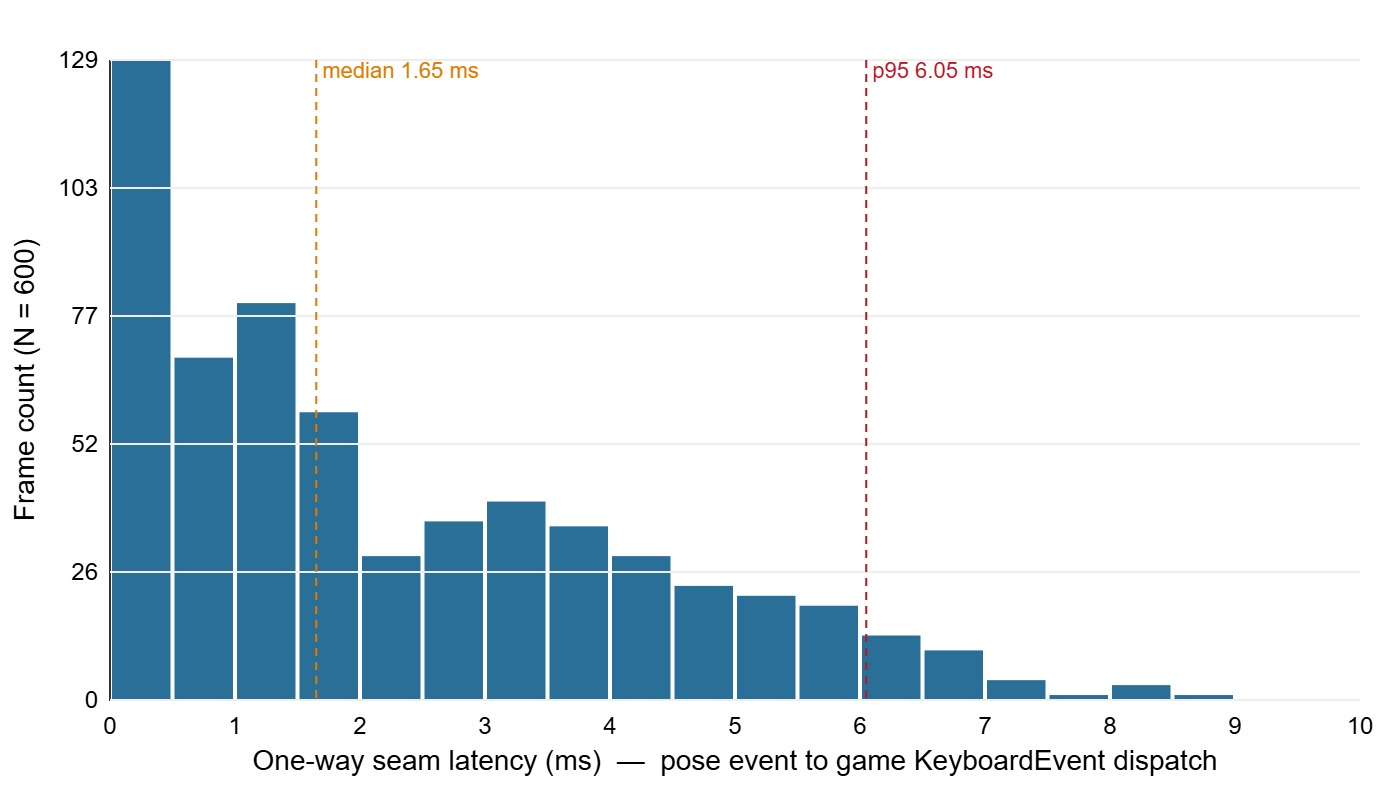
\includegraphics[width=0.78\textwidth]{figures/latency.jpg}
  \caption{Distribution of one-way motion-seam latency (hub \postmsg{} send
  $\to$ in-iframe receipt, immediately preceding \texttt{KeyboardEvent}
  dispatch) over $N=600$~frames, measured while a Phaser~3 game rendered
  concurrently. Median $1.65$\,ms; 95th percentile $6.05$\,ms; all samples
  well within the $16.7$\,ms 60\,fps frame budget.}
  \label{fig:latency}
  \vspace{-1.0em}
\end{figure}

\noindent\emph{Threat to construct validity:} this micro-benchmark isolates
the \postmsg{} transport, which dominates the seam's marginal cost; it does
not include the upstream MediaPipe inference time (a property of the sensing
black box, evaluated in the companion paper~\citecompanion{}) nor the
downstream in-engine input dispatch.

\subsection{E4: Design-Principle Walkthrough}

Each design principle is satisfied by concrete implementation evidence.
\textbf{DP1:} only \texttt{PoseDetector} calls \texttt{getUserMedia}; the bridge
stubs out \texttt{poseDetector.init()} inside iframes.
\textbf{DP2:} six discrete events plus ten continuous hold states are exposed;
games never parse raw landmarks.
\textbf{DP3:} all seven games run with zero lines of gameplay code changed,
against $\approx$230~shared bridge$+$coach LOC.
\textbf{DP4:} two engines coexist behind the same seam, with
hub$\leftrightarrow$game isolation and independent load/unload.
\textbf{DP5:} rPPG and the difficulty controller each expose a single scalar, so
internal replacement does not affect any game.

% =========================================================================
\section{Discussion: Transdisciplinary Reflection}
\label{sec:discussion}
% =========================================================================

The seam architecture concretely enables independent disciplinary
evolution.
\paragraph{Swap the vision model (Discipline 1):} Replace MediaPipe
Pose with a newer skeleton estimator (e.g., a transformer-based
model). Only \texttt{PoseDetector.processPosture()} changes; the
\motionbus{}, bridge, and all seven games are untouched.
\paragraph{Add physiological sensing (Discipline 2):} The rPPG
estimator was added late in development. It registers as a
listener on \texttt{PoseDetector}, emits \texttt{bpm} and
\texttt{confidence} to the HUD. No game was modified.
\paragraph{Plug in a new game engine (Discipline 4):} The Three.js
Hoverboard game was added after the Phaser games. Integration
required only a 2-entry \motionmap{} and two script includes.
\paragraph{Replace the difficulty controller (Discipline 2):}
The \texttt{DifficultyController} could be swapped for a
reinforcement-learning agent. It communicates with games solely
through the \texttt{MOTION\_DIFFICULTY} scalar on the
\texttt{control} channel.
\paragraph{Add coaching without touching games (Discipline 3):}
The \texttt{Coach} cue system and \texttt{MoveDemo} stick-figure
display were developed independently and plugged in via the
\texttt{expectMove} message.

These examples demonstrate that the seam is not merely a software
interface---it is the mechanism that \emph{operationalizes
transdisciplinary integration}, allowing experts in each discipline to
contribute without understanding or modifying the others.

\paragraph{Generalizable principles.}
Three principles generalize beyond exergaming to transdisciplinary
human-in-the-loop systems. (1)~\emph{Seam-first design:} identify discipline
boundaries \emph{before} implementation---the
Discipline$\times$Concern$\times$Design-Response table
(Table~\ref{tab:transmap}) is a reusable planning artifact. (2)~\emph{Translate,
don't modify:} integrate an artifact from another discipline (a game, a sensor
model, a control law) through a translation layer that adapts its native
interface rather than editing its internals, preserving artifact integrity and
disciplinary autonomy. (3)~\emph{Scalar contracts at boundaries:} reduce complex
internal state to minimal scalar signals (effort $\in [0,1]$, difficulty
$\in [0.85,1.2]$, BPM $\in \mathbb{N}$) at the seam, minimizing coupling and
making substitution feasible.

\subsection{Limitations and Threats to Validity}

Several factors limit the generalizability of our findings.
\paragraph{Internal validity:} The formative evaluation is
author-conducted; independent replication and user studies
(the companion paper's scope) are needed.
\paragraph{External validity:} All games are authored in-house.
Third-party game integration would more strongly test DP3's
``minimal touch'' claim; the zero-LOC-changed evidence is
encouraging but limited to our games.
\paragraph{Construct validity:} Seam latency is measured in a
controlled desktop environment; mobile or low-end hardware may
show different profiles.
\paragraph{Sensing accuracy:} rPPG and pose-detection accuracy are
not evaluated here (companion paper scope).

% =========================================================================
\section{Conclusion and Future Work}
\label{sec:conclusion}
% =========================================================================

This paper presented \sys{}, a browser-based markerless motion-exergaming
platform, and its central contribution: a \emph{transdisciplinary seam
architecture} that decouples six normally entangled disciplines---computer
vision, control, HCI, game design, exercise science, and software
engineering---through a layered design of normalized events, translation
bridges, and scalar contracts.

Grounded in Design Science Research, we derived five design principles
(DP1--DP5), instantiated them in a concrete architecture comprising
\texttt{PoseDetector}, \motionbus{}, \motionbridge{}, and the
\postmsg{} seam, and evaluated them formatively: seven heterogeneous
games across two engines (Phaser~3 and Three.js) are motion-controlled
through a single webcam with no wearables and no modification to their
gameplay code.

The architecture's transdisciplinary value lies not in any single
subsystem, but in the \emph{stable interfaces} that allow each
discipline to evolve independently---a concrete operationalization of
the transdisciplinary integration that SDPS advocates.

\textbf{Future work} includes: empirical user studies evaluating exercise
efficacy, adherence, and player experience (the companion journal
paper~\citecompanion{}); integration of additional game engines (e.g.,
Godot HTML5 exports); exploration of multi-player motion-exergaming; and
investigation of on-device ML-based gesture customization for
accessibility.

% =========================================================================
% REFERENCES
% =========================================================================
\bibliographystyle{splncs04}
\bibliography{references}

\end{document}
